\documentclass[border=4pt,12pt]{standalone}
% House style for redrawn exam diagrams (diagram-v4: 0.4pt lines, filled -latex arrows, fine dashes; stipple and hatching drawn as real dots/lines (no PDF/SVG patterns, so they render in every browser and at any scale); transparent background). Every figure \input's this.
\usepackage{amsmath,amssymb}
\usepackage{txfonts}
\usepackage{pdfrender,xcolor}
% \halo{text}: label on shading. The shading stops just around each letter's outline (a thin knock-out that follows the
% glyphs, like the papers' typesetting), never a box. Owner: "I don't want a box around the text".
\newcommand{\halo}[1]{\leavevmode\rlap{\pdfrender{TextRenderingMode=2,LineWidth=2.2pt,LineJoinStyle=1,StrokeColor=white,FillColor=white}#1}#1}
\usepackage{tikz,pgfplots}
\pgfplotsset{compat=1.18}
\usetikzlibrary{arrows.meta,calc,angles,quotes,patterns,patterns.meta,intersections,positioning,decorations.markings,shapes.geometric}
% Stipple and hatching are drawn as actual dots / lines clipped to the region (path picture), NOT as pattern fills:
% SVG <pattern> fills vanish or blur when browsers scale the image, so the owner could not see the shading.
% Each dot is a 0.72pt square (keeps SVGs small; reads as a dot at print size). Dots sit on one global staggered grid, so neighbouring regions line up.
\makeatletter
\newdimen\ex@x \newdimen\ex@y \newdimen\ex@xa \newdimen\ex@ya \newdimen\ex@xb \newdimen\ex@yb \newcount\ex@row
\def\exam@stipplecolor{black!75}\def\exam@dotr{0.42pt}\def\exam@dotgap{2.5}
\def\ex@rowdots{\ifdim\ex@x<\ex@xb \pgfpathrectangle{\pgfqpoint{\dimexpr\ex@x-0.36pt\relax}{\dimexpr\ex@y-0.36pt\relax}}{\pgfqpoint{0.72pt}{0.72pt}}\advance\ex@x by \exam@dotgap pt\relax\expandafter\ex@rowdots\fi}
\def\exam@stipple{%
  \pgftransformreset% dots are sized in real points even inside scaled pictures
  \pgfpointanchor{path picture bounding box}{south west}\ex@xa=\pgf@x \ex@ya=\pgf@y
  \pgfpointanchor{path picture bounding box}{north east}\ex@xb=\pgf@x \ex@yb=\pgf@y
  \pgfsetfillcolor{\exam@stipplecolor}\pgfmathsetmacro\ex@h{\exam@dotgap/2}%
  \pgfmathtruncatemacro\ex@r{floor(\ex@ya/\ex@h)-1}\ex@row=\ex@r\relax
  \ex@y=\ex@r\dimexpr\ex@h pt\relax
  \loop\ifdim\ex@y<\ex@yb
    \pgfmathtruncatemacro\ex@c{floor(\ex@xa/\exam@dotgap)-1}\ex@x=\ex@c\dimexpr\exam@dotgap pt\relax
    \ifodd\ex@row \advance\ex@x by \ex@h pt\fi
    \ex@rowdots
    \advance\ex@y by \ex@h pt \advance\ex@row by 1
    \ifnum\numexpr\ex@row-(\ex@row/4)*4\relax=0 \pgfusepath{fill}\fi% flush every 4 rows: bounded TeX memory, few clip copies in the SVG
  \repeat\pgfusepath{fill}}
\newdimen\ex@d
\def\exam@hatch#1{% #1 = 1 for /, -1 for \ ; lines 45 degrees, 3pt apart
  \pgftransformreset
  \pgfpointanchor{path picture bounding box}{south west}\ex@xa=\pgf@x \ex@ya=\pgf@y
  \pgfpointanchor{path picture bounding box}{north east}\ex@xb=\pgf@x \ex@yb=\pgf@y
  \ex@d=\dimexpr\ex@yb-\ex@ya\relax \ex@x=\dimexpr\ex@xa-\ex@d\relax
  \loop\ifdim\ex@x<\ex@xb
    \ifnum#1>0 \pgfpathmoveto{\pgfqpoint{\ex@x}{\ex@ya}}\pgfpathlineto{\pgfqpoint{\dimexpr\ex@x+\ex@d\relax}{\ex@yb}}%
    \else \pgfpathmoveto{\pgfqpoint{\ex@x}{\ex@yb}}\pgfpathlineto{\pgfqpoint{\dimexpr\ex@x+\ex@d\relax}{\ex@ya}}\fi
    \advance\ex@x by 4.24pt
  \repeat
  \pgfsetlinewidth{0.4pt}\pgfsetstrokecolor{black}\pgfusepath{stroke}}
\def\examstipple{\exam@stipple}\def\examhatch{\exam@hatch}\def\examsetstipplecolor#1{\def\exam@stipplecolor{#1}}\def\examsetdotgap#1{\def\exam@dotgap{#1}}
\makeatother
% (legacy pattern kept for old files)
% staggered stipple like the NESA papers' dotted shading
\pgfdeclarepatternformonly{exam stipple}{\pgfpointorigin}{\pgfqpoint{2.2pt}{2.2pt}}{\pgfqpoint{2.2pt}{2.2pt}}{%
  \pgfpathcircle{\pgfqpoint{0.55pt}{0.55pt}}{0.42pt}\pgfpathcircle{\pgfqpoint{1.65pt}{1.65pt}}{0.42pt}\pgfusepath{fill}}
\tikzset{
  every picture/.style={line width=0.6pt, >={Latex[length=2mm,width=1.3mm]}},
  curve/.style={line width=0.6pt},
  open arrow/.style={-{Latex[length=2mm,width=1.3mm]}},  % owner: filled -latex heads everywhere, no open chevrons
  aux/.style={dash pattern=on 2pt off 1.5pt, line width=0.6pt},
  shade/.code={\def\exA{#1}\def\exB{none}\ifx\exA\exB\else\pgfkeysalso{fill=black!18}\fi},
  shade/.default=on,
  shade dots/.style={fill=none, path picture={\examstipple}},
  stipple color/.code={\examsetstipplecolor{#1}},
  stipple gap/.code={\examsetdotgap{#1}},
  shade dense dots/.style={fill=none, stipple gap=1.6, path picture={\examstipple}},
  shade hatch/.style={fill=none, path picture={\examhatch{1}}},
  shade hatch reverse/.style={fill=none, path picture={\examhatch{-1}}},
  shade solid/.style={fill=black},
  pt/.style={circle, fill, inner sep=1.1pt},
  open pt/.style={circle, draw, fill=white, inner sep=1.1pt},
}
\pgfplotsset{
  exam axes/.style={axis lines=middle, axis line style={->}, xlabel={$x$}, ylabel={$y$},
    xlabel style={anchor=west}, ylabel style={anchor=south}, tick label style={font=\small},
    every axis plot/.append style={line width=0.6pt, black}, samples=200, clip=false,
    enlargelimits=false, axis on top},
}

\begin{document}
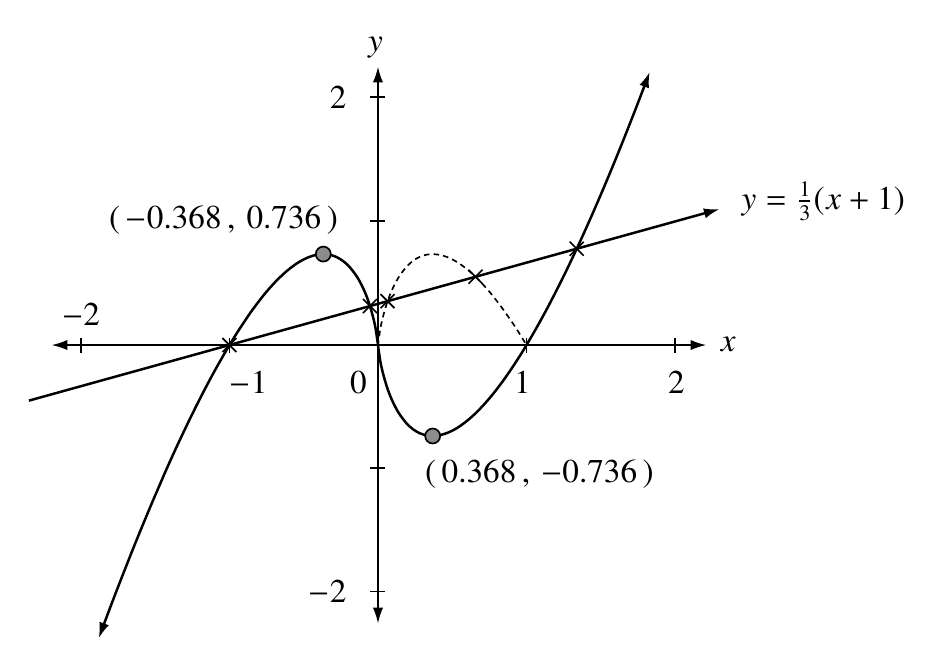
\begin{tikzpicture}[x=0.0127cm,y=-0.0127cm,font=\large]
  \draw[<->] (31,311.5) -- (686,311.5);
  \draw[<->] (357.5,590) -- (357.5,33);
  \foreach \i in {60.5,209,506,654.5}{\draw (\i,304) -- (\i,319);}
  \foreach \j in {63.5,187.5,434.5,558}{\draw (350,\j) -- (365,\j);}
  \node[anchor=base] at (60.5,292) {$-2$};
  \node[anchor=base] at (228,360) {$-1$};
  \node[anchor=base] at (338,360) {$0$};
  \node[anchor=base] at (502,360) {$1$};
  \node[anchor=base] at (656,360) {$2$};
  \node[anchor=east] at (336,63.5) {$2$};
  \node[anchor=east] at (336,558) {$-2$};
  \node at (355,14) {$y$};
  \node at (707,311) {$x$};
  \draw[<->,line width=0.9pt] plot[smooth] coordinates {(78.1,604.9) (84.7,587.1) (91.3,569.6) (97.9,552.4) (104.5,535.5) (111.1,518.8) (117.7,502.4) (124.3,486.4) (130.9,470.6) (137.5,455.2) (144.0,440.1) (150.6,425.3) (157.2,410.9) (163.8,396.9) (170.4,383.2) (177.0,369.9) (183.6,357.0) (190.2,344.5) (196.8,332.5) (203.4,320.9) (210.0,309.7) (216.6,299.1) (223.2,289.0) (229.7,279.4) (236.3,270.4) (242.9,261.9) (249.5,254.1) (256.1,247.0) (262.7,240.6) (269.3,235.0) (275.9,230.1) (282.5,226.2) (289.1,223.2) (295.7,221.3) (302.3,220.6) (308.8,221.1) (315.4,223.2) (322.0,227.0) (328.6,232.8) (335.2,241.2) (337.7,245.1) (340.1,249.5) (342.6,254.5) (345.1,260.2) (347.6,266.8) (350.0,274.3) (352.5,283.2) (355.0,294.3) (357.4,310.6) (357.5,311.5) (357.6,312.4) (360.0,328.7) (362.5,339.8) (365.0,348.7) (367.4,356.2) (369.9,362.8) (372.4,368.5) (374.9,373.5) (377.3,377.9) (379.8,381.8) (386.2,390.0) (392.6,395.8) (399.0,399.6) (405.4,401.7) (411.8,402.4) (418.2,401.9) (424.6,400.2) (431.0,397.6) (437.4,394.0) (443.8,389.5) (450.2,384.3) (456.6,378.3) (463.0,371.6) (469.4,364.3) (475.8,356.4) (482.2,347.9) (488.6,338.8) (495.0,329.2) (501.4,319.2) (507.8,308.6) (514.2,297.6) (520.6,286.2) (527.0,274.4) (533.4,262.1) (539.8,249.5) (546.2,236.5) (552.6,223.1) (559.0,209.4) (565.4,195.3) (571.8,180.9) (578.2,166.2) (584.6,151.2) (591.0,135.9) (597.4,120.3) (603.8,104.4) (610.2,88.2) (616.6,71.8) (623.0,55.1) (629.4,38.1)};
  \draw[aux] plot[smooth] coordinates {(357.5,311.5) (357.6,310.6) (360.0,294.3) (362.5,283.2) (365.0,274.3) (367.4,266.8) (369.9,260.2) (372.4,254.5) (374.9,249.5) (377.3,245.1) (379.8,241.2) (385.1,234.3) (390.3,229.1) (395.6,225.2) (400.8,222.7) (406.1,221.1) (411.4,220.6) (416.6,220.9) (421.9,221.9) (427.2,223.7) (432.4,226.1) (437.7,229.2) (442.9,232.8) (448.2,237.0) (453.5,241.7) (458.7,246.9) (464.0,252.5) (469.3,258.5) (474.5,265.0) (479.8,271.9) (485.0,279.1) (490.3,286.7) (495.6,294.6) (500.8,302.9) (506.1,311.5)};
  \draw[->,line width=0.9pt] (8.3,367.1) -- (699.3,175.5);
  \node[anchor=west] at (711.3,167.5) {$y=\frac{1}{3}(x+1)$};
  \draw (208.9,311.5) ++(-7,-7) -- ++(14,14) ++(0,-14) -- ++(-14,14); \draw (349.5,272.5) ++(-7,-7) -- ++(14,14) ++(0,-14) -- ++(-14,14); \draw (367.1,267.6) ++(-7,-7) -- ++(14,14) ++(0,-14) -- ++(-14,14); \draw (455.1,243.2) ++(-7,-7) -- ++(14,14) ++(0,-14) -- ++(-14,14); \draw (556.3,215.2) ++(-7,-7) -- ++(14,14) ++(0,-14) -- ++(-14,14);
  \filldraw[fill=black!45] (302.8,220.5) circle (7.5) (412.2,402.5) circle (7.5);
  \node at (203,187) {$(\,-0.368\,,\,0.736\,)$};
  \node at (519,441) {$(\,0.368\,,\,-0.736\,)$};
\end{tikzpicture}
\end{document}
